\section{Background}
\subsection{Definitions}
In this work, we focus on mining subgraphs on an labeled data graph $G=\{V,E,\Sigma,L_V,L_E\}$, where $V$ is a set of vertices, $E$ is a set of edges, $\Sigma$ is a set of labels, $L_V$ is a function that associates a vertex $v \in V$ with a label $L_V \in \Sigma$, and $L_E$ is a function that associates an edge $e \in E$ with a label $L_E \in \Sigma$.

\noindent
\textbf{Definition 1 \emph{(Subgraph Matching)}} A graph $g=\{V_g,E_g,\Sigma_g,L_{V_g},L_{E_g}\}$ is isomorphic to a query graph $q=\{V_q,E_q,\Sigma_q,L_{V_q},L_{E_q}\}$, if and only if there exists a bijective function $f: V_q \rightarrow V_g$ such that (1) $\forall u \in V_q$, $f(u) \in V_g$ and $L_{V_q}(u) = L_{V_g}(f(u))$; and (2) $\forall e_q=(u,u') \in E_q$, $e_g=(f(u),f(u')) \in E_g$ and $L_{E_q}(e_q)=L_{E_g}(e_g)$. Subgraph matching is to find all subgraphs (called embeddings) of a data graph $G$ that are isomorphic to a query graph $q$.

\noindent
\textbf{Definition 2 \emph{(Matching Order)}} Given a query graph $q$, a matching order $\pi$ is a permutation of vertices in $q$, and $\pi[i]$ is the $i$th vertex in $\pi$.

\noindent
\RV{\textbf{Definition 3 \emph{(Partial Embedding)}} Given a query graph $q$ and a matching order $\pi$, the subgraph matching will match query vertices along $\pi$ iteratively. Before reaching the end of $\pi$, the matched query vertices and edges constitute a sub-query graph of $q$, which we call the partial query. The subgraphs of a data graph $G$ that are isomorphic to the partial query are called partial embeddings.}

\noindent
\textbf{Definition 4 \emph{(Backward Edge)}} Given a query graph $q$ and a partial query graph $q'$ of $q$, if an edge $e$ exists in $q$ but not in $q'$ and $e$ connects two vertices of $q'$, we call $e$ the backward edge.

\begin{figure}
\centering
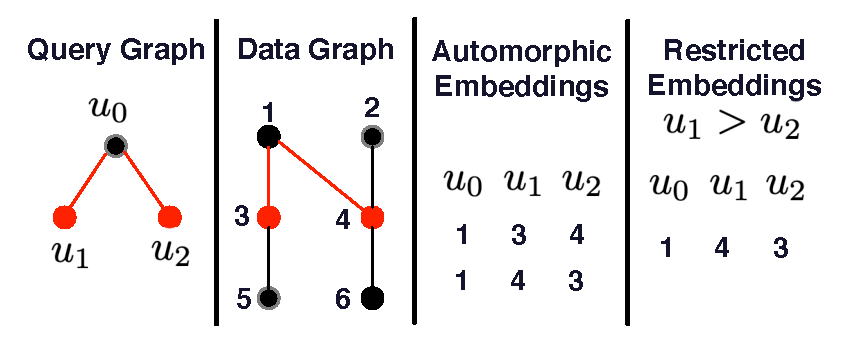
\includegraphics[width=\columnwidth]{./figure/automorphism.eps}
\caption{Examples of automorphic and non-automorphic embeddings.}	
\label{fig:automo}
\end{figure}

If a query graph is symmetric, multiple embeddings can be isomorphic to the same subgraph of a data graph. As shown in Figure \ref{fig:automo}, the query graph has two symmetric vertices, $u_1$ and $u_2$ and two isomorphic embeddings. We can see in Figure \ref{fig:automo} that the two embeddings are the same subgraph of the data graph. To eliminate redundant embeddings, GraphPi \cite{shi2020graphpi} and GraphZero \cite{mawhirter2019graphzero} generate restrictions on query vertices and the corresponding data vertices in each embedding. Figure \ref{fig:automo} shows that with the restriction $u_1 > u_2$, we can eliminate the redundant embedding. We use the same method as GraphPi and GraphZero to break the symmetry of a query graph.

\subsection{GPU Architecture}
GPU has been used in many areas to accelerate applications. The popularity of GPU is primarily attributed to its massive parallelism. To support such large-scale parallelism, GPU employs a complex execution pipeline and memory hierarchy. Modern GPUs usually consist of multiple Streaming Multiprocessors (SMs), and each SM contains multiple Single-Instruction-Multiple-Thread (SIMT) units. Threads in the same SIMT unit are called a warp, the smallest scheduling unit in GPU. The thread-local registers are the fastest memory component, having the lowest access latency (1-2 cycles). The SM local L1 caches and shared memory provide a larger storage capacity over the thread- local registers but have modestly higher accessing latency of around 30 cycles. The off-chip global memory, similar to the RAM in a CPU system, provides the largest memory storage capacity on the GPU but has the longest accessing latency of around 500 cycles.

CUDA provides atomic functions to perform a read-modify-write atomic operation on one 32-bit or 64-bit word residing in global or shared memory. In this work, we use $atomicAdd$ function to read a variable in global memory and add a number to it, and write the result back to the same address.

